\section{表の挿入}
本節では、表の挿入に関して記述する。
また、表の作成方法や書式の変更方法についても実例を元に解説する。

\subsection{表の作成と変換方法}
馴れてくれば \LaTeX の命令を直接記述して表を作るのは容易だが、最初の内は手こずるかもしれない。
ここでは論文に用いる一般的な表を元に、一番簡単と思われる作成と貼り付けの方法を記載する。

\subsubsection{表の作成}
図\ref{fig:tableFinish}の様な表を仕上がりのイメージと仮定する。
\begin{figure}[H]
\centering
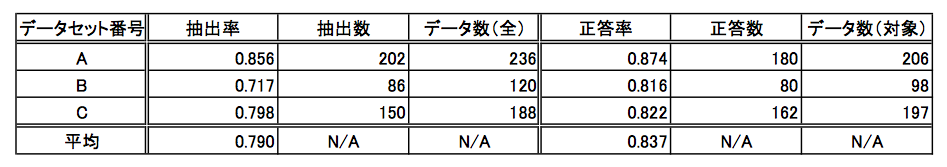
\includegraphics[width=14cm]{tableFinishImage.png}
\vspace{-3mm}
\caption{貼り付けたい表の仕上がりのイメージ}
\label{fig:tableFinish}
%\vspace{2mm}
\end{figure}

まず、Excel等で表を作成しておく。
\begin{figure}[H]
\centering
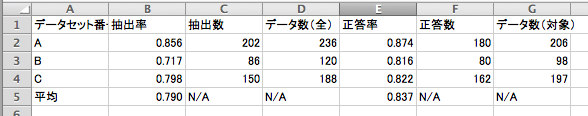
\includegraphics[width=14cm]{excelTable.png}
\vspace{-3mm}
\caption{Excelで作成した表}
\label{fig:excelTable}
%\vspace{2mm}
\end{figure}

\subsubsection{表の変換}
CSV2TeX(\url{http://naisodewafurenu.web.fc2.com/csv2tex.html})に接続する。
\begin{figure}[H]
\centering
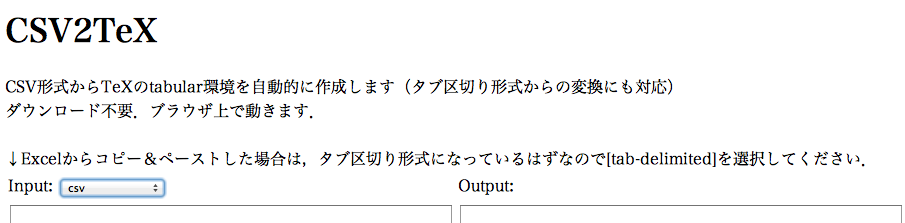
\includegraphics[width=12cm]{csv2tex.png}
\vspace{-3mm}
\caption{CSV2TeXのサイト}
\label{fig:csv2tex}
%\vspace{2mm}
\end{figure}

Inputのプルダウンメニューから「tab-delimited」を選択する。
\begin{figure}[H]
\centering
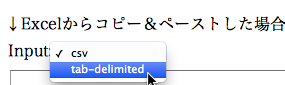
\includegraphics[width=6.5cm]{inputTypeChange.png}
%\vspace{-3mm}
\caption{入力方式の変更}
\label{fig:inputTypeChange}
%\vspace{2mm}
\end{figure}



その直下のボックスにExcelの表をペーストし、「CONVERT」ボタンを押下する。
Outputのボックス内に \LaTeX の表組みの命令が埋め込まれたデータが出力される。
%\begin{figure}[htb]
%\begin{center}
%\includegraphics[height=4cm]{sc02.png}
%\vspace{-3mm}
%\end{center}
%\caption{Excelの表の例}
%\label{fig:excel}
%\vspace{2mm}
%\end{figure}
\begin{figure}[htb]
\centering
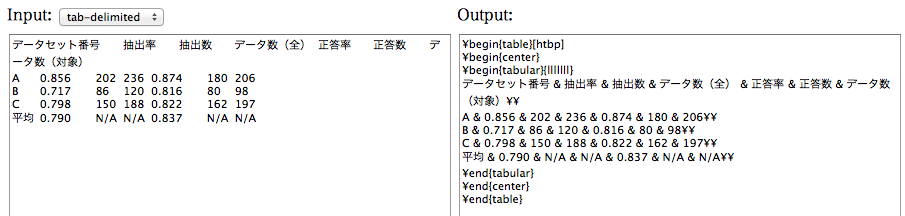
\includegraphics[width=14cm]{convertTable.png}
%\vspace{-3mm}
\caption{CSV2TeXの操作例}
\label{fig:convertTable}
%\vspace{2mm}
\end{figure}

これをtexファイルに貼り付ける。
\begin{breakbox}
{\small
\begin{verbatim}
\begin{table}[htbp]
\begin{center}
\begin{tabular}{lllllll}
データセット番号 & 抽出率 & 抽出数 & データ数(全) & 正答率 & 正答数 & データ数(対象)\\
A & 0.856 & 202 & 236 & 0.874 & 180 & 206\\
B & 0.717 & 86 & 120 & 0.816 & 80 & 98\\
C & 0.798 & 150 & 188 & 0.822 & 162 & 197\\
平均 & 0.790 & N/A & N/A & 0.837 & N/A & N/A\\
\end{tabular}
\end{center}
\end{table}
\end{verbatim}
}
\end{breakbox}

\subsubsection{表の修正}
このままでは、キャプションとラベルが不足しているので、それらの情報を足すことにする。
また、現在の\LaTeX では、図表内において \verb+\begin{center}+と\verb+\end{center}+の代わりに\verb+\centering+命令を使うことが推奨されている為、それも変更する。

まず、命令の上部
\begin{breakbox}
{\small
\begin{verbatim}
\begin{table}[htbp]
\begin{center}
\begin{tabular}{lllllll}
\end{verbatim}
}
\end{breakbox}
に対して、以下の様に修正する。
\begin{breakbox}
{\small
\begin{verbatim}
\begin{table}[htbp]
\caption{実験1の結果}
\centering
\begin{tabular}{lllllll}
\end{verbatim}
}
\end{breakbox}

また、命令下部
\begin{breakbox}
{\small
\begin{verbatim}
\end{tabular}
\end{center}
\end{table}
\end{verbatim}
}
\end{breakbox}
に対して、以下の様に修正する。
\begin{breakbox}
{\small
\begin{verbatim}
\end{tabular}
\label{table:resultEx1}
\end{table}
\end{verbatim}
}
\end{breakbox}


その出力を、表 \ref{table:resultEx1a}に示す。
\begin{table}[H]
\caption{実験1の結果}
\centering
\begin{tabular}{lllllll}
データセット番号 & 抽出率 & 抽出数 & データ数(全) & 正答率 & 正答数 & データ数(対象)\\
A & 0.856 & 202 & 236 & 0.874 & 180 & 206\\
B & 0.717 & 86 & 120 & 0.816 & 80 & 98\\
C & 0.798 & 150 & 188 & 0.822 & 162 & 197\\
平均 & 0.790 & N/A & N/A & 0.837 & N/A & N/A\\
\end{tabular}
\label{table:resultEx1a}
\end{table}


\subsection{横罫線の設定}
横罫線には「\verb+\hline+」命令を利用する。
横罫線を引きたい場所で、\verb+\hline+を入力する。二重線を引きたい場合には、\verb+\hline \hline+と記述すれば良い。

例えば、以下の命令を出力すると表\ref{table:resultEx1b}の様に出力される。
\begin{breakbox}
{\small
\begin{verbatim}
\begin{tabular}{lllllll}
\hline
データセット番号 & 抽出率 & 抽出数 & データ数(全) & 正答率 & 正答数 & データ数(対象)\\ \hline \hline
A & 0.856 & 202 & 236 & 0.874 & 180 & 206\\ \hline
B & 0.717 & 86 & 120 & 0.816 & 80 & 98\\ \hline
C & 0.798 & 150 & 188 & 0.822 & 162 & 197\\ \hline \hline
平均 & 0.790 & N/A & N/A & 0.837 & N/A & N/A\\ \hline
\end{tabular}
\end{verbatim}
}
\end{breakbox}

\begin{table}[H]
\caption{実験1の結果}
\centering
\begin{tabular}{lllllll}
\hline
データセット番号 & 抽出率 & 抽出数 & データ数(全) & 正答率 & 正答数 & データ数(対象)\\ \hline \hline
A & 0.856 & 202 & 236 & 0.874 & 180 & 206\\ \hline
B & 0.717 & 86 & 120 & 0.816 & 80 & 98\\ \hline
C & 0.798 & 150 & 188 & 0.822 & 162 & 197\\ \hline \hline
平均 & 0.790 & N/A & N/A & 0.837 & N/A & N/A\\ \hline
\end{tabular}
\label{table:resultEx1b}
\end{table}

「\verb+\begin{tabular}+」の次の行の「\verb+\hline+」だけが記載されている行は、一番上の横罫線を示す。
また表の一行目(見出し)の最後の部分をみると、改行「\verb+\\+」をし、その後に2回罫線を引く「\verb+\hline \hline+」命令が書かれている為、二重罫線が表示されている。
その他の行は、必要に応じて1回または2回の「\verb+\\ \hline+」が記載されている。

\subsection{表内の基本部分の表示位置の変更}
表内の文字の表示位置を制御している命令は、\verb+\begin{tablar}{lllllll}+
の部分である。
この\verb+{lllllll}+は、表が7列(\verb+l+が7個ある)でできており、それらを「\verb+l+:左寄せ」で表示することを意味している。

表内の表示位置の修正としては、表の大部分を占める部分(2行目から4行目のデータが入っている部分)を元に、位置の指定をしていく。
まず、1列目「AとBとC」とかかれた部分の部分は文字情報なので、センタリング「\verb+c+」にする。
また、2列目から7列目は、数値データが入っていることから、右寄せ「\verb+r+」にする。
したがって、位置の指定は、\verb+\begin{tablar}{crrrrrr}+ とすれば良い。
以上の修正をした表を表 \ref{table:resultEx1c}に示す。
\begin{table}[H]
\caption{実験1の結果}
\centering
\begin{tabular}{crrrrrr}
\hline
データセット番号 & 抽出率 & 抽出数 & データ数(全) & 正答率 & 正答数 & データ数(対象)\\ \hline \hline
A & 0.856 & 202 & 236 & 0.874 & 180 & 206\\ \hline
B & 0.717 & 86 & 120 & 0.816 & 80 & 98\\ \hline
C & 0.798 & 150 & 188 & 0.822 & 162 & 197\\ \hline \hline
平均 & 0.790 & N/A & N/A & 0.837 & N/A & N/A\\ \hline
\end{tabular}
\label{table:resultEx1c}
\end{table}

欧文の論文の場合には、表の縦線を入れないことが多い為、以上で表が完成したと考えて良い。

和文の論文に見られる様に、表の縦線を入れこともできるが、縦線を入れたが為に見出しの位置などが気になり、さらなる調整が必要になることが多い。通常は、ここまでで良いだろう。

\subsection{表の参照}
表の環境でもラベルが設定でき、図と同様の手法で参照することができる。例えば、表 \ref{table:resultEx1a}の命令内では、「\verb+\label{table:resultEx1a}+」と設定されているため、「\verb+表 \ref{table:resultEx1a}+」の様に指定すれば 表 \ref{table:resultEx1a} と参照できる。

\subsection{表の位置の設定}
表の位置の設定は、図の位置の設定と同様「\verb+[htbp]+」の様な指定ができる。である。また、floatパッケージを読み込んでいる為、強制的にその場所に出力する「\verb+[H]+」も利用できる。

\subsection{縦罫線の設定と表内見出しなどの位置変更}
縦方向罫線の入れ方と、それに伴う見出しなどの表示位置変更方法について記載する。

\subsubsection{縦罫線の設定}
列の要素のどこに縦罫線を引くのかを「\verb+|+」を使って指示する。
また、2重罫線は「\verb+||+」を利用する。
例えば、今回の仕上がりのイメージでは、1列目と4列目の右が2重罫線、残りと外側が通常の縦罫線だったので、
「\verb+\begin{tabular}{|c||r|r|r||r|r|r|}+」と書く。
\begin{table}[H]
\caption{実験1の結果}
\centering
\begin{tabular}{|c||r|r|r||r|r|r|}
\hline
データセット番号 & 抽出率 & 抽出数 & データ数(全) & 正答率 & 正答数 & データ数(対象)\\ \hline \hline
A & 0.856 & 202 & 236 & 0.874 & 180 & 206\\ \hline
B & 0.717 & 86 & 120 & 0.816 & 80 & 98\\ \hline
C & 0.798 & 150 & 188 & 0.822 & 162 & 197\\ \hline \hline
平均 & 0.790 & N/A & N/A & 0.837 & N/A & N/A\\ \hline
\end{tabular}
\label{table:resultEx1d}
\end{table}

\subsubsection{表内の見出し行などの部分の表示位置の変更}
表の1行目(ラベル部分)は、2行目から4行目と異なり、それぞれの列を説明する言葉が書かれている。
これは、表内右寄せでは無く、センタリングとしたい。

このように書かれている部分を(表示の関係から行を折り返している)
\begin{breakbox}
{\small
\begin{verbatim}
\begin{tabular}{|c||r|r|r||r|r|r|}
\hline
データセット番号 & 抽出率
  & 抽出数 & データ数(全)
  & 正答率 & 正答数
  & データ数(対象)\\ \hline \hline
\end{verbatim}
}
\end{breakbox}
以下の様に変更する。
\begin{breakbox}
{\small
\begin{verbatim}
\begin{tabular}{|c||r|r|r||r|r|r|}
\hline
\multicolumn{1}{|c||}{データセット番号} & \multicolumn{1}{c|}{抽出率}
  & \multicolumn{1}{c|}{抽出数} & \multicolumn{1}{c||}{データ数(全)}
  & \multicolumn{1}{c|}{正答率} & \multicolumn{1}{c|}{正答数}
  & \multicolumn{1}{c|}{データ数(対象)} \\ \hline \hline
\end{verbatim}
}
\end{breakbox}

なお、命令を見て分かるように \verb+multicolmun+命令を利用する際には、罫線情報は再度指定する必要がある。

また、最後の行は「N/A」の文字は表内でセンタリングとしたい。

同様にこのように書かれている部分を(表示の関係から行を折り返している)
\begin{breakbox}
{\small
\begin{verbatim}
平均 & 0.790
  & N/A & N/A
  & 0.837 & N/A
  & N/A\\ \hline
\end{tabular}
\end{verbatim}
}
\end{breakbox}
以下の様に修正する。
\begin{breakbox}
{\small
\begin{verbatim}
平均 & 0.790
  & \multicolumn{1}{c|}{N/A} & \multicolumn{1}{c||}{N/A}
  & 0.837 & \multicolumn{1}{c|}{N/A}
  & \multicolumn{1}{c|}{N/A} \\ \hline
\end{tabular}
\end{verbatim}
}
\end{breakbox}

以上の修正を施すと、表\ref{table:resultEx1e}の様に出力される。

\begin{table}[H]
\caption{実験1の結果}
\centering
\begin{tabular}{|c||r|r|r||r|r|r|}
\hline
\multicolumn{1}{|c||}{データセット番号} & \multicolumn{1}{c|}{抽出率}
  & \multicolumn{1}{c|}{抽出数} & \multicolumn{1}{c||}{データ数(全)}
  & \multicolumn{1}{c|}{正答率} & \multicolumn{1}{c|}{正答数}
  & \multicolumn{1}{c|}{データ数(対象)} \\ \hline \hline
A & 0.856 & 202 & 236 & 0.874 & 180 & 206\\ \hline
B & 0.717 & 86 & 120 & 0.816 & 80 & 98\\ \hline
C & 0.798 & 150 & 188 & 0.822 & 162 & 197\\ \hline
平均 & 0.790
  & \multicolumn{1}{c|}{N/A} & \multicolumn{1}{c||}{N/A}
  & 0.837 & \multicolumn{1}{c|}{N/A}
  & \multicolumn{1}{c|}{N/A} \\ \hline
\end{tabular}
\label{table:resultEx1e}
\end{table}
